\chapter{Géométrie et contraction locale des distances}

\section{Sujet}

\begin{enumerate}
\item
Soit $\mathcal A = \{0,1\}^2$ contenant les quatre points $(0,0)$, $(0,1)$, $(1,0)$, $(1,1)$ de $\mathbb{R}^2$ muni de sa norme $\ell_1$ qu'on note $\lvert\cdot\rvert$. 
Soit $n\geqslant 2$ un entier et $f : \mathcal A \to \mathbb{R}^n$ une application telle que 
\[\forall x,y\in \mathcal A,\quad \lVert f(x) - f(y) \rVert \leqslant \lvert x - y \rvert,\]
où $\lVert \cdot \rVert$ désigne la norme euclidienne de $\mathbb{R}^n$.

Montrer qu'il existe deux points $a,b\in\mathcal A$ qui vérifient
\[\lVert f(a) - f(b)\rVert \leqslant \frac{\sqrt 2} 2 \lvert a - b\rvert.\]
\item 
On considère maintenant l'ensemble $\mathcal B$ constitué des points $(0,0,0)$, $(1,0,0)$, $(0,1,0)$, $(0,0,1)$ de $\mathbb{R}^3$ muni de sa norme $\ell_1$ qu'on note $\lvert\cdot\rvert$. Soit $n\geqslant 2$ un entier et $f : \mathcal A \to \mathbb{R}^n$ une application telle que 
\[\forall x,y\in\mathcal A, \quad \lVert f(x) - f(y) \rVert \leqslant \lvert x - y \rvert,\]
où $\lVert\cdot\rVert$ désigne la norme euclidienne de $\mathbb{R}^n$.

Montrer qu'il existe deux points $a,b\in\mathcal B$ qui vérifient 
\[\lVert f(a) - f(b)\rVert \leqslant \frac{\sqrt 3} 2 \lvert a - b\rvert.\]
\end{enumerate}

\section{Solution du premier exercice}

\begin{enumerate}
\item 
Notons $A,B,C,D$ les images par $f$ de $(0,0)$, $(1,0)$, $(1,1)$ et $(0,1)$ respectivement. L'hypothèse sur $f$ implique que les distances $AB$, $BC$, $CD$ et $DA$ sont inférieures à $1$. Étant donné que $\lvert(1,0) - (0,1)\rvert = \lvert(1,1) - (0,0)\rvert = 2$, le résultat demandé sera prouvé si on parvient à établir que l'une des deux distances $AC$ ou $BD$ est inférieure à $\sqrt 2$. L'imagination se figure bien le résultat : dans le cas d'un carré de côté $1$ les diagonales sont exactement de longueur $\sqrt 2$ ; et si on déforme ce carré pour écarter les sommets $A$ et $C$ sans augmenter les longueurs des côtés, alors $B$ et $D$ doivent se rapprocher.

\begin{center}
\begin{tikzpicture}[scale=1.5]
\draw (0,0) node [below left] {$A$} -- (1,0) node [below right] {$B$} -- (1,1) node [above right] {$C$} -- (0,1) node [above left] {$D$} -- cycle ;
\draw[dashed] (0,0) -- (1,1) ;
\draw[dashed] (0,1) -- (1,0) ;

\draw (3,0.5) node {$\longrightarrow$} ;

\draw (5,-0.05) coordinate (A) node [below left] {$A$} --++ (70:1) coordinate (D) node [above left] {$D$} --++ (5:1) coordinate (C) node [above right] {$C$} --++ (250:1) coordinate (B) node [below right] {$B$} -- cycle ;
\draw[dashed] (A) -- (C) ;
\draw[dashed] (B) -- (D) ;
\end{tikzpicture}
\end{center}
Je propose deux démonstrations que $\min(AC,BD) \leqslant \sqrt 2$.
\begin{enumerate}
\item
On suppose $AC > \sqrt 2$ pour en déduire $BD \leqslant \sqrt 2$.  Soit $I$ le milieu du segment $[AC]$. Pour n'importe quel point $M\in\mathbb{R}^n$, le premier théorème de la médiane (corollaire de l'identité du parallélogramme) amène $IM^2 = \frac 1 2 (AM^2 + BM^2) - \frac 1 4 AC^2$. En particulier pour $M = B$, les données $AC > \sqrt 2$, $AB \leqslant 1$ et $BC \leqslant 1$ amènent $IB^2 \leqslant \frac 1 2$ donc $IB \leqslant \frac{\sqrt 2} 2$. Pour les mêmes raisons $ID \leqslant \frac {\sqrt 2}2$. L'inégalité triangulaire donne alors $BD \leqslant BI + ID \leqslant \sqrt 2$, CQFD. On remarquera qu'à aucune reprise il n'est supposé ni utile que les points $A,B,C,D$ soient coplanaires.
\item 
Pour montrer qu'au moins un des carrés $AC^2$ ou $BD^2$ est inférieur à $2$, il suffit de prouver 
\[AC^2 + BD^2 \leqslant AB^2 + BC^2 + CD^2 + DA^2 \leqslant 4.\]
Pour cela écrivons
\begin{align*}
AC^2 &= \frac 1 2 \left(\left(\vv{AB} + \vv{BC}\right)^2 + \left(\vv{CD} + \vv{DA}\right)^2\right) \\
BD^2 &= \frac 1 2 \left(\left(\vv{BC} + \vv{CD}\right)^2 + \left(\vv{DA} + \vv{AB}\right)^2\right).
\end{align*}
En développant par bilinéarité on trouve
\begin{align*}
\MoveEqLeft AC^2 + BD^2 - (AB^2 + BC^2 + CD^2 + DA^2) \\
&= \vv{AB} \cdot \vv{BC} + \vv{BC} \cdot \vv{CD}
+ \vv{CD} \cdot \vv{DA} + \vv{DA} \cdot \vv{AB} \\
&= (\vv{AB} + \vv{CD}) \cdot (\vv{BC} + \vv{DA}).
\end{align*}
Or $\vv{BC} + \vv{DA} = \vv{BA} + \vv{AC} + \vv{DC} + \vv{CA} = \vv{BA} + \vv{DC} = - (\vv{AB} + \vv{CD})$
donc 
\[AC^2 + BD^2 - (AB^2 + BC^2 + CD^2 + DA^2)  = -(\vv{AB} + \vv{CD})^2 \leqslant 0\]
CQFD.
\end{enumerate}
\item 
Notons $O,A,B,C$ les images par $f$ de $(0,0,0)$, $(1,0,0)$, $(0,1,0)$ et $(0,0,1)$ respectivement. L'hypothèse sur $f$ implique que les distances $OA$, $OB$ et $OC$ sont inférieures à $1$. En remarquant 
\[\lvert(1,0,0) - (0,1,0)\rvert = \lvert(0,1,0) - (0,0,1)\rvert = \lvert(0,0,1) - (1,0,0)\rvert = 2\] le résultat demandé sera prouvé si on parvient à établir qu'une des trois distances $AB$, $BC$ ou $CA$ est inférieure à $\sqrt 3$. À nouveau, c'est une affirmation assez intuitive : imaginons dans une boule de rayon $1$ construire un triangle dont le plus petit côté soit le plus long possible, il semble alors que la meilleure solution soit un triangle équilatéral inscrit dans un grand cercle ; et ce triangle est justement de côté $\sqrt 3$.

\begin{center}
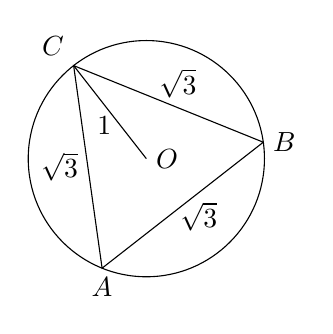
\begin{tikzpicture}[scale=1.5]
\draw (0,0) circle (1) ;
\draw (0,0) node [right] {$O$} -- (128:1) node [pos=0.35,left] {$1$} node [above left] {$C$} ;
\draw (8:1) node [right] {$B$} -- (128:1) node[pos=0.45,above] {$\sqrt 3$} -- (248:1) node[midway,left] {$\sqrt 3$} node [below] {$A$} -- (8:1) node[pos=0.6,below] {$\sqrt 3$} ;
\end{tikzpicture}
\end{center}
Pour prouver cette affirmation, on montre l'égalité suivante en développant les produits scalaires par bilinéarité :
\begin{multline*}
    (\vv{OA} + \vv{OB} + \vv{OC})^2 + (\vv{OB} - \vv{OA})^2 + (\vv{OC} - \vv{OB})^2 + (\vv{OA} - \vv{OC})^2 \\= 3\vv{OA}^2 + 3 \vv{OB}^2 + 3\vv{OC}^2.
\end{multline*}
Il s'ensuit $AB^2 + BC^2 + CA^2 \leqslant 3(OA^2 + OB^2 + OC^2) \leqslant 9$, donc un des trois carrés $AB^2$, $BC^2$ ou $CA^2$ doit être inférieur à $3$, CQFD.
\end{enumerate}

\section{Sujet}

Calculer $$\lim_{A\rightarrow +\infty}I(A):=\frac{1}{A}\int_{1}^{A}A^{\frac{1}{x}}dx.$$

\section{Solution du deuxième exercice}

Soit $A\gg 1.$

On écrit pour $x\geq 1,$ $\displaystyle A^{\frac{1}{x}}=\exp(\frac{1}{x}\ln(A)).$

Ainsi, $$I(A)=\frac{1}{A}\int_{1}^{A}\exp(\frac{1}{x}\ln(A))dx.$$

Un changement de variables donne alors $$I(A)=\frac{\ln(A)}{A}\int_{\frac{\ln(A)}{A}}^{\ln(A)}\frac{e^{u}}{u^{2}}du.$$

Ensuite, on observe : $$\frac{\ln(A)}{A}\int_{\frac{\ln(A)}{A}}^{\ln(A)}\frac{du}{u^{2}}=1-\frac{1}{A}.$$

Considérons $\lambda$ un nombre proche de $1$ par valeur inférieure.

Ainsi, on obtient par l'inégalité triangulaire puis en utilisant l'inégalité des accroissements finis :
\begin{align*}
\vert I(A)-1 \vert  & \leq \frac{1}{A}+\frac{\ln(A)}{A}\int_{\frac{\ln(A)}{A}}^{\ln(A)}\frac{e^{u}-1}{u^{2}}du\\
& \leq \frac{1}{A}+\frac{\ln(A)}{A}\int_{\frac{\ln(A)}{A}}^{\lambda \ln(A)}\frac{e^{u}-1}{u^{2}}du+ \frac{\ln(A)}{A}\int_{\lambda \ln(A)}^{\ln(A)}\frac{e^{u}-1}{u^{2}}du\\
& \leq \frac{1}{A}+\frac{\ln(A)}{A}\times A^{\lambda}\int_{\frac{\ln(A)}{A}}^{\lambda \ln(A)}\frac{u}{u^{2}}du+ \frac{\ln(A)}{A}\times A \int_{\lambda \ln(A)}^{\ln(A)}\frac{du}{u^{2}}du\\
& \leq \frac{1}{A}+\frac{\ln(A)\ln(\lambda A)}{A^{1-\lambda}}+\frac{1}{\lambda}-1.
\end{align*}

Il vient alors par croissances comparées 
$$\limsup_{A\rightarrow +\infty} \vert I(A)-1\vert \leq \frac{1}{\lambda}-1.$$

En faisant tendre $\lambda$ vers $1,$ on obtient le résultat voulu, à savoir : $$\lim_{A\rightarrow +\infty} I(A)=1.$$